%Running title

\pagestyle{fancy} %For main text, if desired: Switch to fancy header
\fancyhead[L]{CHAPTER \thechapter}
%\fancyfoot{}
%\fancyfoot[C]{\thepage}
%\fancyfoot[CO,RE]{Author Name}


\fancyhead[L]{} 
\fancyhead[R]{\small{INTRODUCTION}} 

\nnchap{Introduction}
\setcounter{chapter}{0}
\renewcommand{\thefigure}{\thechapter.\arabic{figure}}

Adaptive behavior requires the flexible use of information to guide actions based on learned contingencies in the environment. In particular, sensorimotor decisions benefit from knowledge of the statistical relationships between sensory cues, actions, and rewarding outcomes. Sensory cues can become instructive when they consistently predict which actions will lead to a favorable outcome. However, these relationships can shift with the environmental context as well as internal states such as hunger or satiety. To select appropriate actions in the face of changing circumstances, the brain must integrate information related to sensory cues as well as past experience and context. How this is accomplished mechanistically remains a question of great scientific interest. 

\nnsec{Role of the Medial Frontal Cortex in Flexible Sensorimotor Behavior}
Goal-directed behavior can be defined as action motivated by the pursuit of a desired outcome. In rodents, the medial frontal cortex (MFC) has been implicated in the representation of task variables that may be crucial for this type of behavior. MFC neurons have been shown to encode information related to recent choices and their outcomes \citep{sul2011role,yuan2015cortical,siniscalchi2019enhanced,mao2019cortical}, as well as upcoming actions \citep{sul2011role,erlich2011cortical,murakami2014neural}. In particular, these studies focused on the most dorsal field of the MFC, which is known as the secondary motor cortex (M2).\footnote{The secondary motor cortex is usually refered to as M2 in mice, but is also called medial agranular cortex(AGm), medial precentral cortex, or the frontal orienting field (FOF) in rats} Within the MFC, M2 neighbors the anterior cingulate cortex (ACC), and receives input from the ACC as well as diverse sensory and association areas \citep{reep1984afferent,reep1999topographic,hoover2007anatomical}. Efferent connections of M2 include the primary motor cortex (M1) and reciprocal connections with the superior colliculus, an anatomical arrangement which would be well-suited for volitional control of spatial orienting movements \citep{erlich2011cortical,barthas2017secondary}. 

\begin{figure}[htbp]

\begin{center}
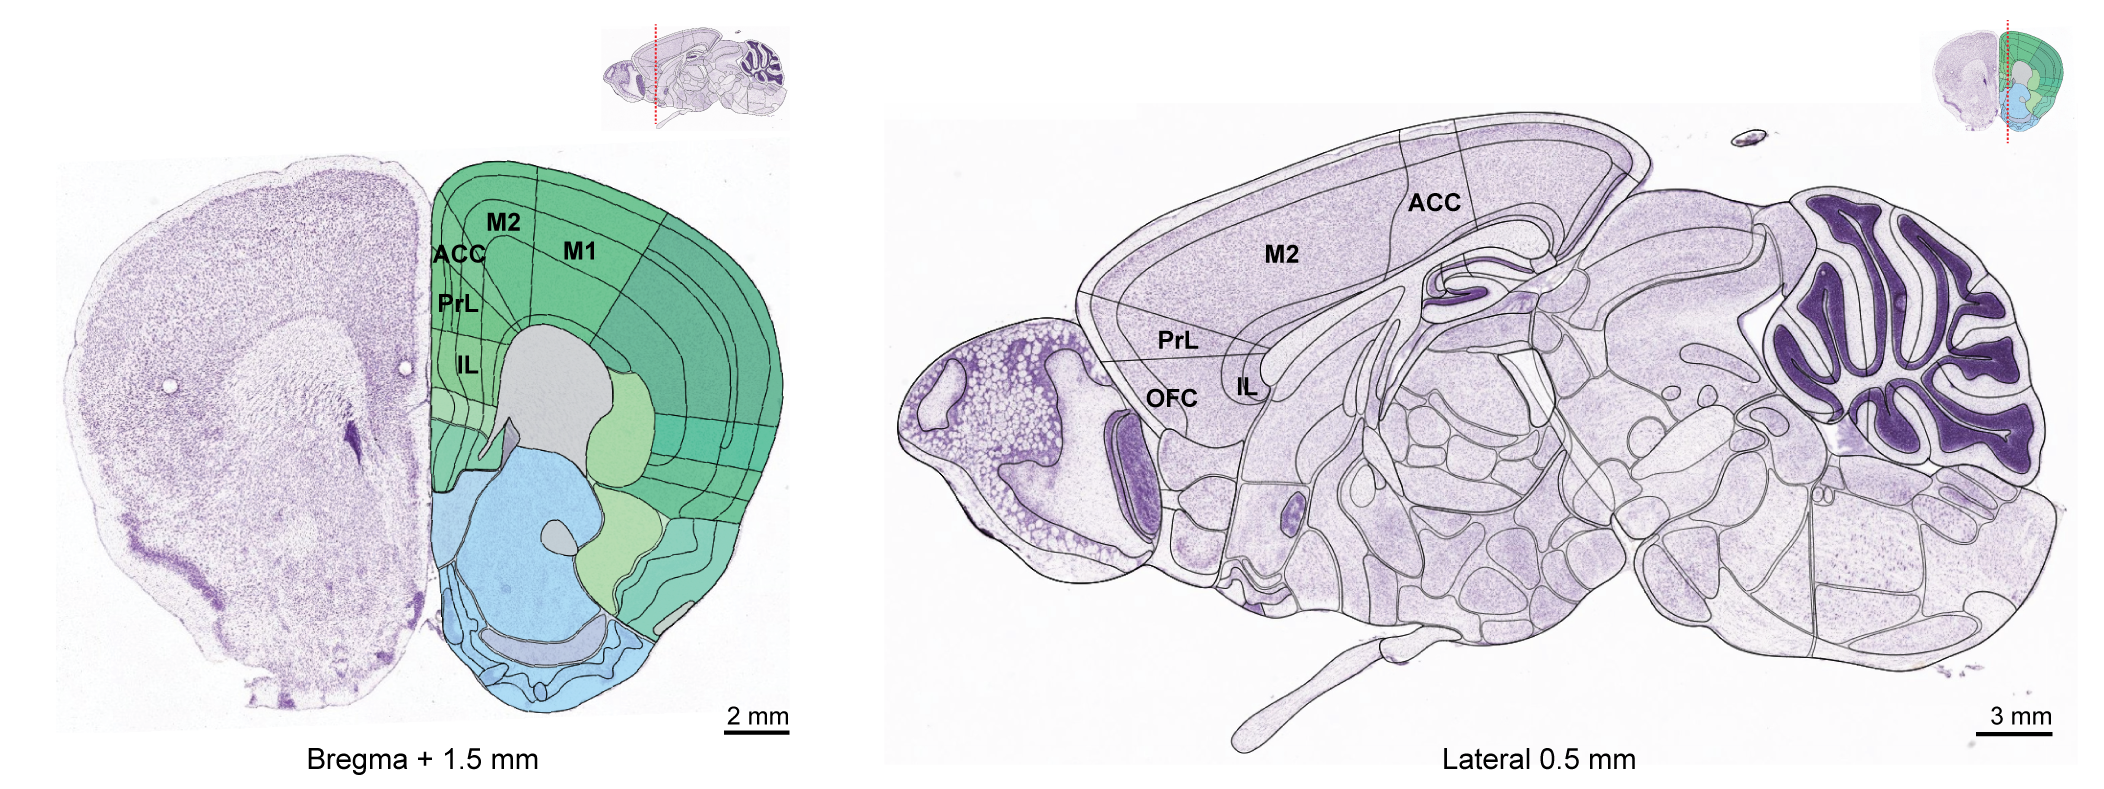
\includegraphics[width=\textwidth]{Figures/Introduction/Intro_fig_M2} 
\end{center}

\caption[Anatomical location of the secondary motor cortex]
{Anatomical location of the secondary motor cortex (M2) in the mouse. The images show an example Nissl-stained coronal (left) and saggital section (right) of the mouse brain containing M2, overlaid with approximate cytoarchitectural boundaries as defined in the Allen Mouse Brain Atlas. The anterior-posterior and medial-lateral coordinates of these sections are indicated by red dashed lines in the insets, and approximate the region of M2 imaged for the experiments in Chapters 1--3. Cortical areas in the coronal section are shaded in green. M1, primary motor cortex. ACC, anterior cingulate cortex including cingulate areas 1--2. PrL, prelimbic cortex. IL, infralimbic cortex. OFC, orbitofrontal cortex. All images were adapted from the Allen Mouse Brain Atlas (\url{https://mouse.brain-map.org/}.}

\label{fig:CC_fig1}
\end{figure}


One recent study demonstrated that signals for an upcoming choice within a figure-eight maze appeared earlier within M2 than in other brain regions including the medial prefrontal and orbitofrontal cortices (mPFC and OFC), M1, and the striatum \citep{sul2011role}. Bilateral lesioning of M2 in the same study impaired decisions based on the outcome of prior choices. Together, these results suggest activity related to action initiation or planning, and may implicate M2 in computations that incorporate the value of alternative spatial targets.  

While information related to prior choices and their outcomes are unnecessary in situations where the task depends only on well-learned stimulus-response relationships, such information may be crucial during value-based decision making, associative learning, or adjustment to changing contingencies in the environment. Consistent with this idea, it was recently demonstrated that modulation of MFC neuronal activity by prior outcomes can predict learning rate in an operant visuomotor task \citep{mao2019cortical}. 

Recent studies have also directly implicated M2 in sensorimotor decisions, using variations on the two-alternative forced-choice task to examine its causal contributions to lateralized decisions informed by either short-term memory \citep{erlich2011cortical,guo2014flow,kopec2015cortical} or the accumulation of sensory evidence \citep{erlich2015distinct,hanks2015distinct}. Unilateral pharmacological \citep{erlich2011cortical} or optogenetic silencing of M2 \citep{hanks2015distinct,kopec2015cortical} was demonstrated to induce an ipsilateral choice bias when rodents were required to make lateralized choices based on arbitrary auditory-motor \citep{erlich2011cortical,kopec2015cortical} or somatosensory-motor associations \citep{guo2014flow}, but not when a visuospatial cue indicated the rewarded choice. These results may provide evidence that the interhemispheric balance of M2 activity can impart a bias on sensorimotor decisions specifically in tasks that require the use of arbitrary associations between sensory cues and actions. 

Neural representations of the behavioral context have also been found in M2 \citep{durstewitz2010abrupt,hyman2012contextual,siniscalchi2016fast} as well as adjacent cortical fields in the mPFC \citep{rich2009rat}. Collectively, these results suggest that MFC may play an important role in the selection or planning of specific actions based on sensory cues, prior reinforcement, and behavioral context. However, we lack a detailed understanding of how cortical microcircuits, including those in MFC, process such information during context-dependent sensorimotor decisions. 

\nnsec{Experimental Framework}
In the next three chapters, we will present three independent studies that attempt to make progress on this question. Each takes a similar reductionist experimental approach to study the neurophysiological correlates of sensorimotor behavior, with the goal of uncovering task-related information content in the activity of MFC neurons. Namely, we leveraged a two-choice sensorimotor decision-making task that can be performed by head-restrained mice under the objective of a two-photon fluorescence microscope used for simultaneously measuring neural activity (Fig. \ref{fig:Intro_ExpSetup}). \begin{SCfigure}[][htbp]

% \begin{center}
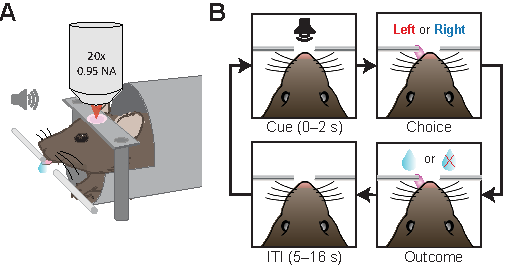
\includegraphics[width=8.7cm]{Figures/Introduction/Intro_fig_ExpSetup} 
% \end{center}
\caption[Experimental framework]
{Common experimental framework for the experiments presented in Chapters 1--3. (A) Experimental apparatus for dual-choice auditory-motor task with simultaneous two-photon imaging. (B) Flow diagram of trial structure. A sound cue was played at the start of each trial, indicating the target spout that would be rewarded (left or right). To obtain the reward, subjects were required to lick the target within 2 s following cue onset. After an intertrial interval (ITI) of 5--16 s, a new sound cue was presented, providing a fresh opportunity to lick for a reward. }


\label{fig:Intro_ExpSetup}
\end{SCfigure}


Two-photon microscopy allows \emph{in vivo} imaging of neurons at cellular resolution using fluorescent dyes or genetically encoded fluorescent proteins. To measure neural activity during our experiments, we expressed the genetically encoded Ca$^{2+}$ indicator GCaMP6 in cortical neurons, typically using an adeno-associated viral vector. GCaMP6 reports the increases in intracellular Ca$^{2+}$ concentration associated with action potentials with large ($\sim 25\%$) increases in fluorescence that can be captured with time-lapse imaging \citep{chen2013ultrasensitive}. To gain optical access to the brain, a section of skull above the M2 region of MFC was replaced with an implanted glass window.

The mouse rested in a modified stainless steel tube throughout the experiment, restrained by an implanted stainless steel head-plate secured to the imaging apparatus. The microscope objective was positioned over M2 and focused to a depth of 175--400 \si{\um} from the brain surface, in order to image cellular fluorescence transients from GCaMP6$^+$ neurons within cortical layers 2/3 while subjects performed the task.

The task consisted of a set of trials in which subjects could choose between two stainless steel water spouts placed on either side of the mouth, only one of which (the target) would provide a water reward on a given trial. A sound cue played through a set of speakers at the start of each trial indicated the target side. The cues were repeated logarithmic chirps of either ascending (upsweeps) or descending mean frequency (downsweeps).  If the target spout was licked within 2 s of cue onset, then it would immediately deliver a small drop of water. After an intertrial interval of 5--16 seconds, the next cue was played, providing the opportunity to make another choice. New trials were generated until the subject failed to choose a spout for twenty consecutive trials. 

The targets indicated by each sound cue varied across different experiments that will be presented in Chapters \ref{CC_paper}--\ref{CellTypes_paper}. However, it is important to note that in all cases the sensorimotor mappings leading to a reward were arbitrary \citep{white1999rule,wise2000arbitrary}---that is, the instructive content of each sensory cue could not be derived from any natural (eg, spatial) relation with the target and had to be learned through trial and error. 

\nnsec{Choices and their Outcomes}
Associations between past choices and their outcomes allow for efficient selection of actions likely to meet one’s present goals. The mechanisms by which such associations are internalized by the nervous system remain unclear. However, at the behavioral level, it is well known that rewarded choices tend to be repeated at the expense of those that have yielded meager or aversive results. 

How does the brain selectively reinforce rewarded actions in order to bias their future implementation? Physiological studies in primates and rodents suggest that the frontal cortex plays an important role in these functions. For example, the primate prefrontal cortex is known to contain neurons that encode chosen actions and outcomes \citep{barraclough2004prefrontal,  genovesio2006representation, seo2007dynamic, histed2009learning}, suggesting a plausible neural substrate for their association during goal-directed behavior. Moreover, single-unit recordings have revealed that prior reward can enhance the discriminability of spiking activity related to past \citep{donahue2013cortical} and upcoming choices \citep{histed2009learning}.

Similarly, recordings from the MFC of rodents have revealed neural signatures of prior choices and their outcomes \citep{sul2010distinct, sul2011role, hyman2017novel}. Murine MFC has also been implicated in the flexible acquisition and initiation of voluntary actions \citep{ostlund2009evidence, gremel2013premotor, murakami2014neural, siniscalchi2016fast, barthas2017secondary, makino2017transformation}. Based on its putative role in instrumental behavior, M2 may serve as an important interface for the mixing of choice- and reward-related signals in the rodent brain. However, the details of how reinforcement might interact with choice-related neural representations remain unclear. 

In Chapter 1, we will explore the associative mechanisms underlying goal-directed action selection, focusing on the question of how populations of simultaneously recorded neurons in the cerebral cortex may represent and integrate information related to choices and their outcomes. One intriguing hypothesis is that a choice’s outcome could affect the strength or persistence of its neural signature in MFC. To test this idea, we trained mice on the two-choice auditory discrimination task shown in Fig. \ref{fig:Intro_ExpSetup} and then introduced a probabilistic reinforcement schedule during the two-photon imaging sessions. In this experiment, upsweeps always indicated a left target and downsweeps always indicated a right target. Three randomly interleaved outcomes (single, double and omitted rewards) delivered when the correct target was chosen allowed us to measure the impact of reward on choice signaling by populations of MFC neurons, as well as to distinguish effects of changes in reward magnitude from those of its absolute presence or absence. 

We found that rewarding outcomes boosted the fidelity of choice signals encoded in the population activity patterns---an effect that persisted into the subsequent trial. Importantly, the reward-dependent enhancement of choice-related signals depended less on differences in reward size than on the categorical presence or absence of rewards. These results suggest one plausible cortical mechanism for the reinforcement of rewarded actions. Namely, rewarding outcomes can lead to a more robust population-level read-out of recent choice history.

\nnsec{Cortical Representations of Behavioral Context}

In constant environments, animals may come to rely on specific sensory cues to guide actions. However, it is sometimes necessary to discard well-established sensorimotor associations when learned contingencies between specific sensory cues, actions, and outcomes break down. For this reason, control of action selection by the nervous system benefits from both stability and flexibility. On the one hand, stability allows the exploitation of regularities to maximize reward. On the other, flexibility enables rapid adjustment when changes in contingencies occur. Balancing stability and flexibility is therefore a key requirement of adaptive decision-making. Importantly, many psychiatric disorders are marked by disruption in the capacity to balance these opposing aspects of cognitive control \citep{griffiths2014translational}.  

How does the brain find the right balance of flexibility and stability in a changing environment? Previous studies have observed changes in the firing rates of individual neurons in multiple frontal cortical regions following a shift in task contingencies \citep{asaad2000task,rich2009rat,rodgers2014neural}. Behavioral adjustment through trial-and-error learning has been associated with gradual changes that generally match or lag the time course of improvements in task performance \citep{mitz1991learning,chen1995neuronal,pasupathy2005different,antzoulatos2011differences}. 

However, neurons in the frontal cortex can exhibit substantial cell-to-cell variability in their rates of activity change as new sensorimotor associations are acquired \citep{mitz1991learning}. Therefore, it may be necessary to record from large populations to adequately capture the circuit dynamics \citep{mante2013context}. Studies using neural ensemble recordings to examine activity dynamics associated with adjustment to changing task contingencies found the transitions in network activity to be surprisingly abrupt \citep{durstewitz2010abrupt,karlsson2012network}. However, the functional significance of these findings may be difficult to assess without quantitative comparisons of transitions in ensemble activity that differ in their dynamics. Network transitions that differ in their relative rates of change, or in their onset with respect to behavioral changes, could reflect distinct underlying mechanisms for adaptive control of behavior.

To study adaptive sensorimotor decision-making in mice, in Chapter \ref{NN_paper} we modified the basic task shown in Figure \ref{fig:Intro_ExpSetup} to include three distinct auditory-motor mappings (rules). Subjects were required to shift among these rules multiple times within a single session. In the sound rule, upsweeps signified a left target, and downsweeps signified a right target as described above for the experiment in Chapter 1. In the action-left rule, the target on every trial was the left spout, regardless of whether upsweeps or downsweeps were presented. Conversely, under the action-right rule, the right spout was always the target, irrespective of the auditory cue. Sessions were structured into alternating blocks of sound and action trials. The number of trials spent in each rule context was determined by a performance criterion: after 20 consecutive trials with $\geq 85\%$  accuracy, a rule switch would occur---ie, a new rule block would begin on the next trial.

We found that distinct population activity patterns were associated with each of the three rules. Moreover, the transitions between activity patterns occurred earlier and were more abrupt during adjustment to the sound rule---when subjects were required to engage learned sensorimotor associations---than during adjustment to the action rule, when subjects were required to disregard these associations. The results of our study may indicate that behavioral adaptation can be associated with distinct neural transition dynamics, depending on how the task constrains possible response strategies in each environment.

\nnsec{Task-Related Activity in Cortical Cell Types}

The rodent MFC may serve an important role in the selection or planning of specific actions based on sensory cues, prior reinforcement, and behavioral context---as argued in numerous studies discussed in the sections above. However, we lack a detailed understanding of how cortical microcircuits, including those in MFC, process such information during context-dependent decisions. One important basic question regards how this labor might be divided among different cell types of the neocortex. 

Neurons of the cerebral cortex are striking in their diversity, and can be classified based on differences in morphology, physiology, connectivity, and molecular markers \citep{connors1990intrinsic,kubota1994three,kawaguchi1995physiological,tremblay2016gabaergic,huang2019diversity}. However, recently developed mouse lines that selectively express cyclic recombinase (cre) in genetically defined cell types \citep{taniguchi11} have focused intense interest on four non-overlapping cell populations that collectively account for $\sim$ 97\% of cortical neurons \citep{tremblay2016gabaergic}: the somatostatin (SST$^+$), parvalbumin (PV$^+$), and vasointestinal peptide-positive (VIP$^+$) GABAergic interneurons, and the excitatory pyramidal neurons, which express the Ca$^{2+}$-calmodulin dependent kinase CaMKII$\alpha$ (PYR; \citep{jones1994alpha,wang2013distribution}).

Based on their subcellular postsynaptic targets, specific classes of GABAergic interneurons may regulate the flow of activity through cortical networks in a highly specialized manner \citep{kepecs2014interneuron}. For example, SST$^+$ interneurons preferentially target the dendrites of PYR cells, and PV$^+$ interneurons preferentially target their cell body and proximal axon. These subcellular anatomical features correspond to the excitatory inputs and outputs, respectively, of the PYR cells, which may project within or outside of the local microcircuit. More broadly, SST- and PV-mediated inhibition might serve to route the information flowing into and out of the processing units within MFC. In contrast to other inhibitory cell-types, VIP$^+$ interneurons almost solely target other interneurons, and make particularly strong synapses on SST neurons. Thus, VIP cells appear to specialize in disinhibition \citep{letzkus2011disinhibitory,pi13,karnani2016opening}, and in particular may disinhibit the dendrites of PYR neurons through their suppression of SST activity.

Recent studies exploring the role of medial prefrontal cell types in goal-directed behavior have revealed a variety of cell type-specific behavioral correlates which may suggest distinct roles in the processing of task-related information. The earliest study of this kind \citep{kvitsiani2013distinct} found that entry into a reward zone positioned at the end of a linear track was punctuated by rapid suppression of activity in a sub-population of SST cells, and reward zone exit was marked by a transient increase in PV activity. Subsequent studies have contrasted two or more of the GABAergic populations with regard to their sensitivity to sensory cues, trial outcomes, motor responses, or upcoming choices \citep{pinto2015cell,kim2016distinct}.

In Chapter \ref{CellTypes_paper} we will examine task-related signaling in four distinct MFC cell types during flexible sensorimotor behavior. In these experiments, we used cell type-specific calcium imaging to measure the activity patterns of SST, VIP, PV, and PYR neurons during the rule switching task described in Chapter \ref{NN_paper}. Our goal was to estimate the contributions of each cell type to the representation of choices, outcomes, and the rules governing reinforcement. We quantified signals for each of these variables at the single-unit level using a modulation index based on the receiver operating characteristic. The results of these analyses implicate all four cell types in the representation of choices and their outcomes, as well as the reinforcement context in which sensorimotor decisions are made. 